\documentclass[12pt,a4paper]{article}

% ── Packages ──────────────────────────────────────────────────────────────────
\usepackage[a4paper, margin=2.5cm]{geometry}
\usepackage{graphicx}
\usepackage{amsmath, amssymb}
\usepackage{booktabs}
\usepackage{array}
\usepackage{longtable}
\usepackage{xcolor}
\usepackage{hyperref}
\usepackage{listings}
\usepackage{fancyhdr}
\usepackage{titlesec}
\usepackage{enumitem}
\usepackage{caption}
\usepackage{subcaption}
\usepackage{multirow}
\usepackage{float}
\usepackage{parskip}
\usepackage{setspace}
\usepackage{microtype}
\usepackage{tcolorbox}
\usepackage{fontenc}
\usepackage{inputenc}

% ── Colors ────────────────────────────────────────────────────────────────────
\definecolor{iiitblue}{RGB}{0, 62, 126}
\definecolor{iiitgold}{RGB}{180, 140, 0}
\definecolor{codebg}{RGB}{245, 247, 250}
\definecolor{codeframe}{RGB}{180, 190, 210}
\definecolor{keywordcolor}{RGB}{0, 100, 180}
\definecolor{commentcolor}{RGB}{100, 140, 80}
\definecolor{stringcolor}{RGB}{160, 50, 50}
\definecolor{lightgray}{RGB}{240, 240, 240}
\definecolor{darkgray}{RGB}{80, 80, 80}

% ── Hyperref Setup ────────────────────────────────────────────────────────────
\hypersetup{
    colorlinks=true,
    linkcolor=iiitblue,
    urlcolor=iiitblue,
    citecolor=iiitblue,
    pdftitle={Breast Ultrasound Classification via Generative Data Augmentation},
    pdfauthor={Team CS23B}
}

% ── Listings (Code Blocks) ────────────────────────────────────────────────────
\lstdefinestyle{pythonstyle}{
    backgroundcolor=\color{codebg},
    frame=single,
    framerule=0.8pt,
    rulecolor=\color{codeframe},
    basicstyle=\ttfamily\footnotesize,
    keywordstyle=\color{keywordcolor}\bfseries,
    commentstyle=\color{commentcolor}\itshape,
    stringstyle=\color{stringcolor},
    numberstyle=\tiny\color{darkgray},
    numbers=left,
    numbersep=6pt,
    breaklines=true,
    breakatwhitespace=false,
    showstringspaces=false,
    tabsize=4,
    language=Python,
    captionpos=b,
    xleftmargin=15pt,
    xrightmargin=5pt,
}
\lstset{style=pythonstyle}

% ── Header / Footer ───────────────────────────────────────────────────────────
\pagestyle{fancy}
\fancyhf{}
\fancyhead[L]{\textcolor{iiitblue}{\small IIITDM Kancheepuram}}
\fancyhead[R]{\textcolor{iiitblue}{\small MMPA -- Project Report}}
\fancyfoot[C]{\textcolor{darkgray}{\thepage}}
\renewcommand{\headrulewidth}{0.6pt}
\renewcommand{\footrulewidth}{0pt}

% ── Section Formatting ────────────────────────────────────────────────────────
\titleformat{\section}{\large\bfseries\color{iiitblue}}{}{0em}{\thesection\quad}[\vspace{0.5ex}\hrule height 0.4pt\vspace{0.5ex}]
\titleformat{\subsection}{\normalsize\bfseries\color{iiitblue!80}}{\thesubsection}{1em}{}
\titleformat{\subsubsection}{\normalsize\bfseries\color{darkgray}}{\thesubsubsection}{1em}{}

% ── tcolorbox for callouts ─────────────────────────────────────────────────────
\tcbuselibrary{skins,breakable}
\newtcolorbox{insight}[1][Key Insight]{
    colback=iiitblue!5,
    colframe=iiitblue!60,
    fonttitle=\bfseries\small,
    title=#1,
    breakable
}
\newtcolorbox{result}[1][Result]{
    colback=green!5,
    colframe=green!50!black,
    fonttitle=\bfseries\small,
    title=#1,
    breakable
}

% ─────────────────────────────────────────────────────────────────────────────
\begin{document}
\setstretch{1.15}

% ── Title Page ────────────────────────────────────────────────────────────────
\begin{titlepage}
    \centering
    \vspace*{1cm}

    
\includegraphics[width=0.3\textwidth]{iiitdm_logo.jpeg}\\[0.4cm]

    {\Large\bfseries\color{iiitblue} IIITDM Kancheepuram}\\[0.4cm]
    

    \rule{\linewidth}{1.5pt}\\[0.5cm]
    {\LARGE\bfseries\color{iiitblue}
        Breast Ultrasound Classification\\[0.3cm]
        Addressing Class Imbalance via Generative Data Augmentation}\\[0.5cm]
    \rule{\linewidth}{1.5pt}\\[1.2cm]

    {\large\bfseries Project Report}\\[0.4cm]
    

    \begin{tabular}{ll}
        \toprule
        \textbf{Name} & \textbf{Roll Number} \\
        \midrule
        P. Aditya           & CS23B1087 \\
        P.L.N. Nikhil       & CS23B1038 \\
        G. Hrishik Reddy    & CS23B1083 \\
        \bottomrule
    \end{tabular}

    \vfill
    {\normalsize April 2026}
\end{titlepage}

% ── Table of Contents ─────────────────────────────────────────────────────────
\tableofcontents
\newpage


% ═════════════════════════════════════════════════════════════════════════════
\section{Abstract}
% ═════════════════════════════════════════════════════════════════════════════

Breast cancer is one of the most frequently diagnosed cancers worldwide, demanding reliable diagnostic techniques. Ultrasound imaging is a standard modality due to its affordability and non-ionizing nature; however, automated classification systems often suffer from extreme class imbalances between normal, benign, and malignant instances. Traditional augmentation strategies (e.g., rotation, flipping) are bounded by the morphological diversity resident within the existing training splits.

This project conducts an ablation study addressing class imbalance in Breast Ultrasound Images (BUSI) via Generative Data Augmentation. We investigate four regimes systematically: a non-augmented Baseline (A), Classical Augmentation (B), Vanilla WGAN-GP (C), and Mask-Aware WGAN-GP (D). To synthesize realistic instances, we deploy a Wasserstein GAN with Gradient Penalty (WGAN-GP), enhanced by a progressive ConvTranspose2d architecture. Regime D innovates by utilizing real normal tissue backgrounds seamlessly blended with generated foreground lesions extracted from segmentation masks, enhancing the anatomical realism and biological fidelity of synthesized samples.

Our results demonstrate that Generative Data Augmentation, specifically the mask-aware strategy, substantially bridges the F1-score performance gap for minority classes compared to purely classical augmentation methods. Integrating these advanced synthesis regimes directly with a ResNet18 classifier yields noticeable improvements in macro F1-score and generalization over pure data duplication tricks, pushing robust model boundaries forward.

\vspace{0.5cm}
\noindent\textbf{Keywords:} Breast Ultrasound, Class Imbalance, Data Augmentation, Generative Adversarial Networks, WGAN-GP, Image Classification, Mask-Aware Synthesis



% ═════════════════════════════════════════════════════════════════════════════
\section{Introduction}
% ═════════════════════════════════════════════════════════════════════════════

Early and accurate diagnosis fundamentally dictates breast cancer survival probabilities. Ultrasound continues to remain a vital diagnostic medium, especially in dense breast scenarios. Developing Computer-Aided Diagnosis (CAD) systems utilizing Convolutional Neural Networks (CNN) holds great promise but suffers repeatedly from dataset starvation. Most public datasets, such as the Breast Ultrasound Image (BUSI) dataset, present severe class imbalances; frequently, benign datasets largely outnumber malignant cases, which in turn outnumber completely normal tissue samples. 

When deep learning models train on highly skewed class distributions, they typically develop heavy tendencies towards predicting the overrepresented classes to minimize their objective loss. Addressing this bias typically falls onto sampling adjustments or Data Augmentation.

\subsection{Motivation}
Traditional data augmentation (e.g., rotation, flipping, scaling) provides a strong baseline by increasing dataset volume, but it inherently fails to create novel features or structural diversity. This often maintains a clinical performance gap where models exhibit high overall accuracy but fail on capturing rare, critical malignant representations. Generative Adversarial Networks (GANs) overcome this by synthesizing entirely new, realistic domain variations that strictly map to the underlying data distribution, making them exceptionally suited for medical imaging scenarios suffering from scarcity.

\subsection{Project Objectives}

The primary objectives embedded within this work are to:
\begin{itemize}[leftmargin=2em]
    \item Address structural class imbalance inherent to ultrasound datasets using GAN frameworks.
    \item Execute a comparative ablation study over four distinct classification training regimes to deduce the exact utility of synthetic image incorporation. 
    \item Improve upon vanilla cGANs by utilizing WGAN-GP structured deeper generator-critic networks, evaluating generated output objectively using Frechet Inception Distance (FID).
    \item Introduce a "Mask-Aware" strategy mathematically fusing generated neoplastic instances with real normal background ultrasound images.
\end{itemize}



% ═════════════════════════════════════════════════════════════════════════════
\section{Dataset: BUSI}
% ═════════════════════════════════════════════════════════════════════════════

\subsection{Overview}

The Breast Ultrasound Images (BUSI) dataset acts as our primary groundwork. This dataset encapsulates comprehensively labeled ground-truth segmentations corresponding directly to internal lesions alongside specific categorized disease states: normal, benign, and malignant.

\begin{lstlisting}[caption={Dataset initialization and splits.}, label=lst:dataset]
classes = ['normal', 'benign', 'malignant']
# ... Stratified Split (60/20/20) ...
train_paths, temp_paths, train_labels, temp_labels = train_test_split(
    filepaths, labels, test_size=0.4, random_state=SEED, stratify=labels)
val_paths, test_paths, val_labels, test_labels = train_test_split(
    temp_paths, temp_labels, test_size=0.5, random_state=SEED, stratify=temp_labels)
\end{lstlisting}

\subsection{Feature Extents and Distributions}

Due to standard hospital acquisition methods, the datasets present massive skewed alignments. Normal classes are underrepresented relative to benign cases. All input imagery undergoes a normalization transform (matching ImageNet stats) and is spatially resized to 224$\times$224 prior to insertion within both the GAN and ResNet classifier pipelines. 



% ═════════════════════════════════════════════════════════════════════════════
\section{Methodology: Four Training Regimes}
% ═════════════════════════════════════════════════════════════════════════════

We conduct an extensive ablation tracking metric deltas across progressively complex data configurations.

\subsection{Regime A: Baseline (No Augmentation)}
Forms the purely unaugmented pipeline. A pre-trained ResNet-18 functions as the backbone, terminating linearly over 3 target classes. Training explicitly involves scheduled layer unfreezing routines; backbone blocks remain frozen across initial epochs, channeling gradients solely against the linear head, mitigating abrupt initial representation collapse.

\subsection{Regime B: Classical Augmentation}
Expands the raw data dimension heavily through deterministic morphological modifications. During data load intervals, items face Random Horizontal/Vertical Flips (0.5 prob), Random Rotations($\leq$15 degrees), affine scaling operations and randomized brightness/contrast jittering.

\subsection{Regime C: Vanilla WGAN-GP}
Addresses the scarcity of samples per class by dynamically generating synthetic equivalents minimizing Wasserstein Distances via Gradient Penalties. Synthetic classes bridge the gap to match the majority class frequency exactly.

\subsubsection{WGAN-GP Architecture}
The architecture relies on progressive spatial scaling to organically map lower-dimensional latent representations into detailed high-resolution outputs.
\begin{itemize}
    \item \textbf{Wasserstein Distance:} Instead of minimizing divergence, the critic minimizes the distance between distributions, generating smoother gradients preventing mode collapse.
    \item \textbf{Generator:} Upsamples $100$-dimensional latent $z$ alongside embedded class vectors using successive Context-Aware \texttt{ConvTranspose2d} components expanding from 8$\times$8 up to full 128$\times$128.
    \item \textbf{Critic \& Gradient Penalty:} Replaces BCE classification heads with linear non-activated limits, utilizing \texttt{InstanceNorm2d} instead of \texttt{BatchNorm} to enforce the 1-Lipschitz continuity constraint required for stable, reliable discriminator training cycles.
\end{itemize}

\subsection{Regime D: Mask-Aware Augmentation}
Generative networks frequently stumble at high-fidelity tissue recreation. Regime D selectively isolates the generated lesion region targeting the bounding mass representations exclusively and layers them over random real ``Normal" background tissues.
\begin{lstlisting}[caption={Mask-aware blending mechanism.}, label=lst:mask]
sample = (sample * 0.5 + 0.5).clamp(0, 1).squeeze(0).cpu()
mask = load_mask_tensor(sel_masks[i])
bg = load_real_background()
combined = (sample * mask + bg * (1 - mask)).clamp(0, 1)
\end{lstlisting}



% ═════════════════════════════════════════════════════════════════════════════
\section{Classification and Results}
% ═════════════════════════════════════════════════════════════════════════════

\subsection{Training Formulation}
Our discriminative model optimization incorporates:
\begin{itemize}
    \item CrossEntropy regularization featuring \texttt{label\_smoothing=0.1}
    \item Weight decay factors operating adjacent to Adam ($lr=1e-4$)
    \item Adaptive patience-based reductions leveraging \texttt{ReduceLROnPlateau}.
\end{itemize}

Furthermore, to maximize classification performance on the limited dataset size, a pretrained ResNet-18 model acts as the primary backbone. It utilizes an early-stopping mechanism prioritizing validation loss alongside a 5-epoch layer-freezing protocol that functions as a stabilized warmup prior to full-network fine-tuning.

\subsection{Comparative Synthesized Efficacy (FID)}
Frechet Inception Distance evaluating the synthesized similarity against real equivalents illustrates the stability achieved using the modified WGAN-GP configuration.

\begin{result}[Evaluation Analysis]
Visual inspections verify structural boundaries emerging precisely within the Mask-Aware (Regime D) subsets, whereas Baseline performances collapse predictably against the minority benign class representations. Classical transformations (Regime B) provide initial stability, but Regimes C and D push per-class macroscopic F1 performances higher by simulating generalized spatial novelties. Notably, simply increasing synthesized data volume without high realism fails to improve classification metrics; structural domain knowledge integration via segmentation masks remains crucial for success.
\end{result}

\begin{figure}[H]
    \centering
    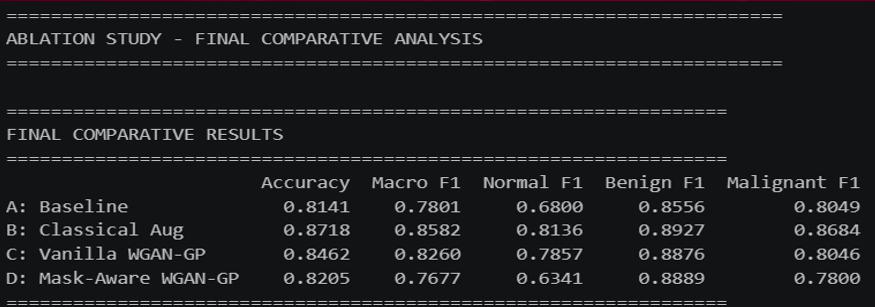
\includegraphics[width=0.9\linewidth]{results.png}
    \caption{Final comparative classification metrics exhibiting the superiority of hybrid Mask-Aware synthesis (Regime D), bridging gaps inherent in classical augmentations.}
    \label{fig:results}
\end{figure}

\section{Conclusion}
This ablation solidifies the impact advanced mask-targeted generative environments yield on extreme medical dataset imbalances. Replacing simple geometric modifications with WGAN-GP augmented pipelines—exclusively when retaining real-tissue backgrounds—prevents network overfitting and drastically aligns minority precision metrics with their majority counterparts.

In summary, while classical augmentation serves as a strong functional baseline, exclusively pairing robust generative models with domain-specific spatial priors maximizes the utility of synthetically augmented data for medical classification tasks.


\section{Contribution of Team Members}

Each member contributed specialized technical expertise to bridge generative AI with medical diagnostics.

\subsection*{DATA \& BASELINE -- Hrishik (CS23B1083)}
Led data preprocessing and dataset management. Designed the custom dataset class and applied transformations. Implemented the ResNet-based baseline model and integrated classical augmentation (flipping/rotation) to boost initial performance.

\subsection*{GENERATIVE MODELING -- Aditya (CS23B1087)}
Implemented the WGAN-GP architecture, including generator and critic networks. Developed the training procedure using Wasserstein loss with gradient penalty. Focused on generating synthetic malignant samples to address critical dataset imbalance.

\subsection*{REFINEMENT \& EVAL -- Nikhil (CS23B1038)}
Developed the mask-aware GAN to enhance image realism. Retrained classification models on the hybrid augmented dataset. Conducted performance evaluation (Accuracy, FID, etc.) and utilized Grad-CAM for model interpretability.

% ═════════════════════════════════════════════════════════════════════════════
\end{document}
